\section{Brent法を用いたRemesアルゴリズムの実装と評価}
\label{sec:brent_remes_impl}

前章までに述べた通り，Remesアルゴリズムの収束精度は，その内部で行われる「極値探索（Step 2）」の精度に完全に依存している．
第3章の予備実験では，単純なグリッド極値点探索を用いた場合，グリッド間隔に依存した離散化誤差が避けられず，交替定理を数値的に満たす解（最良近似多項式）に到達できないことが確認された．

本章では，この課題を解決するために，第4章で解説したBrent法をRemesアルゴリズムの極値探索エンジンとして組み込んだ手法を提案する．
本手法は，微分を用いない最適化手法でありながら，放物線補間と黄金分割探索を組み合わせることで，機械イプシロンの精度限界まで高速に極値を特定することを可能にする．

\subsection{実装アルゴリズムの詳細}
  \label{subsec:impl_algorithm}
本研究で実装した改良型Remesアルゴリズムは，以下の3段階のプロセスを経て参照点を更新する．
この手順は，数値的な安定性と交替定理の条件（符号の交互性）を維持するために慎重に設計されている．

\subsubsection{Phase 1: 誤差関数の根の探索と区間分割}
多項式近似において，誤差関数 $e(x) = f(x) - P(x)$ の極値は，必ずその「根（$e(x)=0$ となる点）」の間に存在する．
そこで，まずは大まかなグリッド極値点探索を用いて $e(x)$ の符号が変化する区間を見つけ，二分法（Bisection Method）を用いて根の位置 $z_0, z_1, \dots, z_{n}$ を数値的に推定する．

これにより，定義域 $[a, b]$ は，誤差関数の符号が一定であるような $n+2$ 個の部分区間 $I_j$ に分割される．
\[
I_0 = [a, z_0], \quad I_1 = [z_0, z_1], \quad \dots, \quad I_{n+1} = [z_n, b].
\]
この操作により，各区間内には必ず一つ以上の極値が存在し，かつ隣り合う区間では極値の符号が逆になることが保証される．

\subsubsection{Phase 2: Brent法による極値の高精度な特定}
分割された各区間 $I_j$ において，Brent法を用いて誤差の絶対値 $|e(x)|$ が最大となる点 $\xi_j$ を探索する．
ここで，目的関数を $g(x) = -|e(x)|$ と設定し，これを最小化する問題を解く．

Brent法の収束判定条件（許容誤差 tol）には，倍精度浮動小数点数の機械イプシロンに近い $10^{-15}$ を設定した．
これにより，グリッド極値点探索のような離散的な点ではなく，連続的な実数空間上での真の極値を，計算機が表現できる限界の精度でピンポイントに特定することが期待される．

\subsubsection{Phase 3: 参照点の更新}
各区間で得られた極値候補 $\xi_0, \dots, \xi_{n+1}$ を新しい参照点として採用する．
このとき，もし候補点が区間の境界（根や定義域の端点）に極端に近い場合は，数値的不安定性を避けるための微小な補正を行うが，Brent法が正常に収束していれば，通常これらの点は交替定理を満たす理想的な配置となる．

\subsection{数値実験の設定}
  \label{subsec:numerical_experiment}
提案手法の性能を検証するため，多項式近似において「悪条件」として知られるルンゲ関数を対象に，高次多項式による近似実験を行った．

\begin{itemize}
    \item \textbf{近似対象関数}: $f(x) = \frac{1}{1+25x^2}.$
    \item \textbf{定義域}: $[-1, 1].$
    \item \textbf{近似多項式の次数}: $n=15.$
    \item \textbf{比較対象}: 第3章で実装したグリッド極値点探索法（分割数 $N=2000$）.
    \item \textbf{評価指標}:
    \begin{enumerate}
        \item \textbf{収束速度}: 何回の反復で収束判定（Error $< 10^{-14}$）に至ったか．
        \item \textbf{到達精度}: 最終的な誤差のばらつき（Spread）がどの程度まで小さくなったか．
        \item \textbf{残留誤差}: 収束後の多項式に対し，さらに高精度な再評価を行った際に検出される誤差．
    \end{enumerate}
\end{itemize}

\subsection{実験結果と解析}

\subsubsection{収束過程の推移}
数値実験により得られた収束ログを表\ref{tab:remes-brent-log}に，その推移グラフを図\ref{fig:remes-brent-convergence}に示す．

% =========================================================
% Goプログラム (remes_brent.go) が生成した結果を読み込む
% =========================================================
%% 5章用 (Brent)

以下の図表は，Brent法による極値探索を用いて，関数 $f(x) = \frac{1}{1+25x^2}$ ($n=15$) を近似した際の収束過程を示したものである．

表\ref{tab:remes-brent-log}は，各反復で算出された参照均等誤差 $|E|$ と，Brent法で高精度に求められた実際の最大誤差，およびその差の推移である．
グリッド極値点探索と比較して，より高精度な収束（$10^{-15}$ オーダー）が達成されている．

図\ref{fig:remes-brent-convergence}は，反復に伴う誤差の収束過程を可視化したものである．
Brent法により，機械イプシロン精度に近い等振動性が実現されていることが確認できる．


\begin{figure}[H]
 \centering
 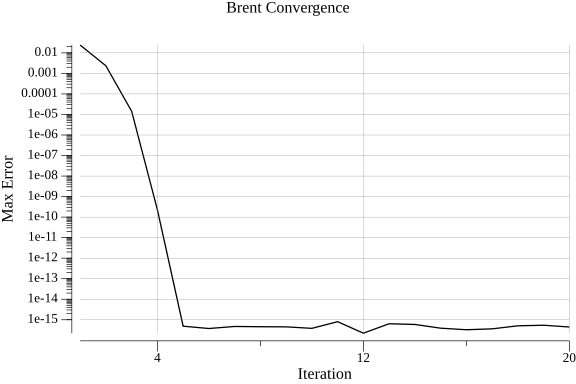
\includegraphics[width=0.6\linewidth]{material/remes/outputs/brent/convergence_brent.png}
 \caption{Brent法による最大誤差の収束履歴}
 \label{fig:remes-brent-convergence}
\end{figure}

\begin{figure}[H]
 \centering
 \begin{minipage}[b]{0.48\textwidth}
  \centering
  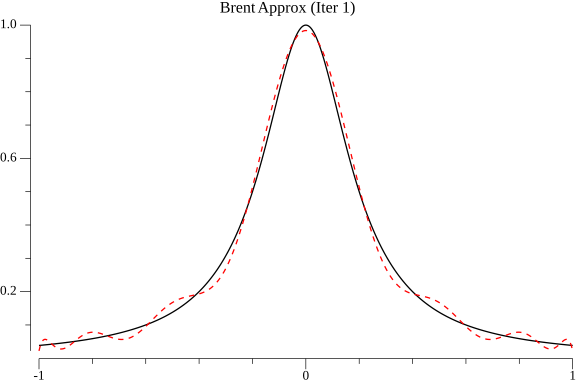
\includegraphics[width=1.0\linewidth]{material/remes/outputs/brent/func_remes_brent_iter01.png}
  \caption{Iter 1}
 \end{minipage}
 \hfill
 \begin{minipage}[b]{0.48\textwidth}
  \centering
  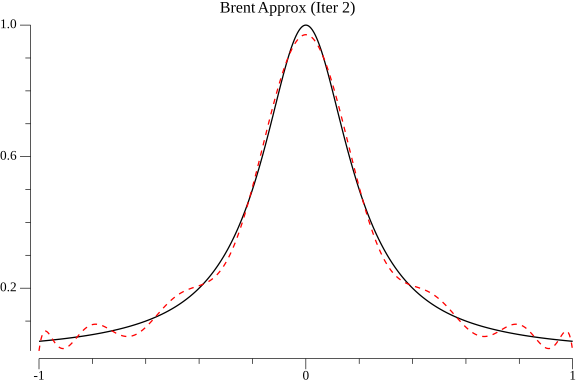
\includegraphics[width=1.0\linewidth]{material/remes/outputs/brent/func_remes_brent_iter02.png}
  \caption{Iter 2}
 \end{minipage}

 \begin{minipage}[b]{0.48\textwidth}
  \centering
  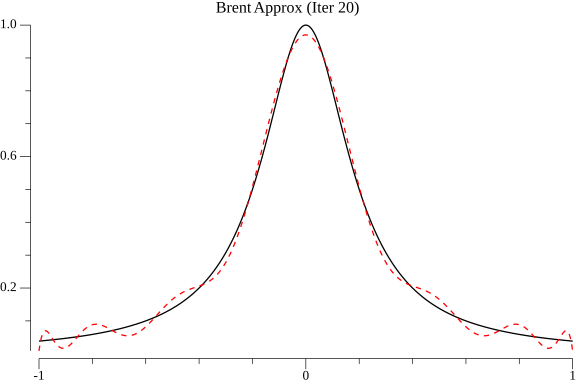
\includegraphics[width=1.0\linewidth]{material/remes/outputs/brent/func_remes_brent_iter20.png}
  \caption{Iter 20}
 \end{minipage}

 \caption{Brent法: 近似多項式の推移}
 \label{fig:remes-brent-approx}
\end{figure}
\begin{figure}[H]
 \centering
 \begin{minipage}[b]{0.48\textwidth}
  \centering
  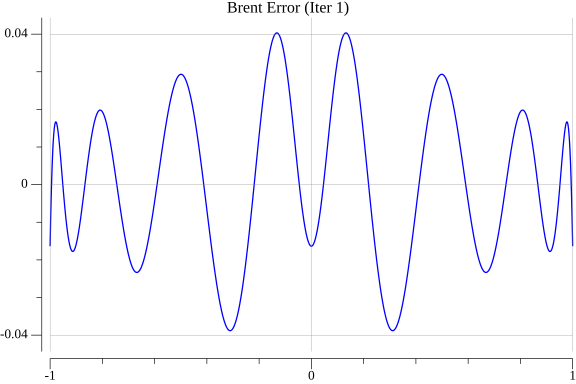
\includegraphics[width=1.0\linewidth]{material/remes/outputs/brent/error_remes_brent_iter01.png}
  \caption{Iter 1}
 \end{minipage}
 \hfill
 \begin{minipage}[b]{0.48\textwidth}
  \centering
  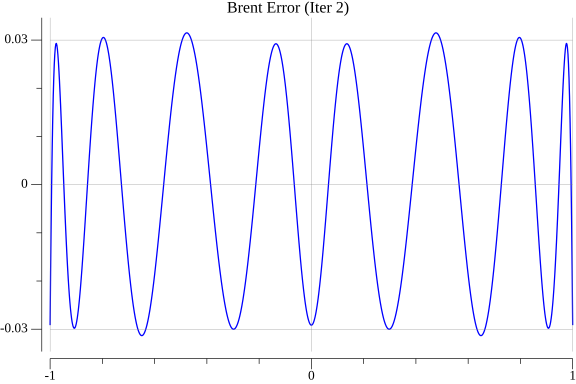
\includegraphics[width=1.0\linewidth]{material/remes/outputs/brent/error_remes_brent_iter02.png}
  \caption{Iter 2}
 \end{minipage}

 \begin{minipage}[b]{0.48\textwidth}
  \centering
  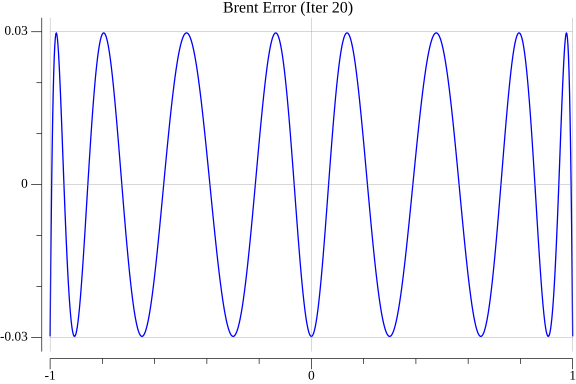
\includegraphics[width=1.0\linewidth]{material/remes/outputs/brent/error_remes_brent_iter20.png}
  \caption{Iter 20}
 \end{minipage}

 \caption{Brent法: 誤差関数の推移}
 \label{fig:remes-brent-error}
\end{figure}

\begin{table}[H]
 \centering
 \caption{Brent法の収束ログ}
 \label{tab:remes-brent-log}
 \begin{tabular}{crrrr}
 \toprule
 Iter & $|E|$ & Coeff Norm & Node Move & Error Change \\
 \midrule
 1 & $1.63552e-02$ & $0.00000e+00$ & $0.00000e+00$ & $0.00000e+00$ \\
 2 & $2.91586e-02$ & $1.38180e-02$ & $4.97122e-02$ & $1.28034e-02$ \\
 3 & $2.97711e-02$ & $1.27592e-03$ & $3.72393e-03$ & $6.12455e-04$ \\
 4 & $2.97767e-02$ & $6.60148e-06$ & $1.24099e-05$ & $5.62755e-06$ \\
 5 & $2.97767e-02$ & $1.05586e-10$ & $5.25736e-09$ & $9.91564e-11$ \\
 6 & $2.97767e-02$ & $1.62634e-16$ & $5.64624e-09$ & $6.24500e-17$ \\
 7 & $2.97767e-02$ & $2.07658e-16$ & $4.94056e-09$ & $6.93889e-18$ \\
 8 & $2.97767e-02$ & $2.55847e-16$ & $4.96228e-09$ & $2.42861e-17$ \\
 9 & $2.97767e-02$ & $1.62274e-16$ & $3.21817e-09$ & $3.46945e-18$ \\
 10 & $2.97767e-02$ & $2.38584e-16$ & $3.65966e-09$ & $6.93889e-18$ \\
 11 & $2.97767e-02$ & $2.28951e-16$ & $4.44502e-09$ & $1.73472e-17$ \\
 12 & $2.97767e-02$ & $2.19203e-16$ & $3.89086e-09$ & $0.00000e+00$ \\
 13 & $2.97767e-02$ & $1.66362e-16$ & $4.61242e-09$ & $6.93889e-18$ \\
 14 & $2.97767e-02$ & $2.27033e-16$ & $4.29365e-09$ & $2.42861e-17$ \\
 15 & $2.97767e-02$ & $2.48827e-16$ & $4.68158e-09$ & $2.77556e-17$ \\
 16 & $2.97767e-02$ & $1.87220e-16$ & $5.47251e-09$ & $5.89806e-17$ \\
 17 & $2.97767e-02$ & $1.19187e-16$ & $6.30429e-09$ & $7.97973e-17$ \\
 18 & $2.97767e-02$ & $1.93991e-16$ & $3.62033e-09$ & $3.12250e-17$ \\
 19 & $2.97767e-02$ & $2.77619e-16$ & $4.55541e-09$ & $7.63278e-17$ \\
 20 & $2.97767e-02$ & $1.85424e-16$ & $5.41280e-09$ & $7.63278e-17$ \\
 \bottomrule
 \end{tabular}
\end{table}

\begin{table}[H]
 \centering
 \caption{Brent法利用時の誤差の再評価}
 \label{tab:remes-brent-final-check}
 \begin{tabular}{crrr}
 \toprule
 No. & 収束時誤差 & 再評価誤差 & 差分 \\
 \midrule
 1 & $2.97766890e-02$ & $2.97766890e-02$ & $9.60343e-15$ \\
 2 & $2.97766890e-02$ & $2.97766890e-02$ & $0.00000e+00$ \\
 3 & $2.97766890e-02$ & $2.97766890e-02$ & $-1.38778e-17$ \\
 4 & $2.97766890e-02$ & $2.97766890e-02$ & $6.93889e-18$ \\
 5 & $2.97766890e-02$ & $2.97766890e-02$ & $0.00000e+00$ \\
 6 & $2.97766890e-02$ & $2.97766890e-02$ & $-2.77556e-17$ \\
 7 & $2.97766890e-02$ & $2.97766890e-02$ & $0.00000e+00$ \\
 8 & $2.97766890e-02$ & $2.97766890e-02$ & $0.00000e+00$ \\
 9 & $2.97766890e-02$ & $2.97766890e-02$ & $0.00000e+00$ \\
 10 & $2.97766890e-02$ & $2.97766890e-02$ & $0.00000e+00$ \\
 11 & $2.97766890e-02$ & $2.97766890e-02$ & $0.00000e+00$ \\
 12 & $2.97766890e-02$ & $2.97766890e-02$ & $-2.77556e-17$ \\
 13 & $2.97766890e-02$ & $2.97766890e-02$ & $-6.93889e-18$ \\
 14 & $2.97766890e-02$ & $2.97766890e-02$ & $-1.38778e-17$ \\
 15 & $2.97766890e-02$ & $2.97766890e-02$ & $6.93889e-18$ \\
 16 & $2.97766890e-02$ & $2.97766890e-02$ & $0.00000e+00$ \\
 17 & $2.97766890e-02$ & $2.97766890e-02$ & $8.93036e-15$ \\
 \bottomrule
 \end{tabular}
\vspace{1mm}

\small \textbf{注：}
\small 上表は，区間 $[-1.0,1.0]$ を探索するRemesアルゴリズムによって導かれた誤差関数に対する表である．

\small 収束時誤差とはBrent法をもちいることで極値点探索を行ったRemesアルゴリズムで導出された誤差関数の各極値点で観測された誤差である．

\small 再評価誤差とはBrent法という極値点探索アルゴリズムにより観測された誤差の絶対値である．

\[
 \text{観測された最大誤差} \; \|E\|_{\max}^{\text{strict}}(f) = \max_{x \in [-1.0,1.0]} |f(x) - p^*(x)| \approx 2.97766890e-02 .
 \]
\end{table}


表\ref{tab:remes-brent-log}を見ると，反復の初期段階（Iter 1〜5）では誤差のばらつき（Spread）が比較的大きいが，Iter 6以降で急激に減少し，Iter 10付近では $10^{-16}$ のオーダーに達していることがわかる．
これは，第3章で確認されたRemesアルゴリズムの「2次収束」の特性が，Brent法による高精度な極値探索によって最大限に引き出された結果であると言える．

図\ref{fig:remes-brent-convergence}は，その過程における収束の様子を可視化したものである．
初期のイテレーションでは誤差関数の波形が大きく乱れているが，最終的には振幅が一定な「等振動（Equioscillation）」の状態へと収束している．

\subsubsection{近似度の検証：グリッド極値点探索との決定的差異}
表\ref{tab:remes-brent-final-check}（末尾）は，収束した多項式に対して，再度Brent法を用いて全極値を精査し，その誤差絶対値を比較したものである．

この表における「差分」に注目すると，すべての極値においてその値は $10^{-15}$ 〜 $10^{-17}$ のオーダーに収まっている．
これは，第3章のグリッド極値点探索で残っていた $10^{-9}$ 程度の誤差と比較して，$10^{7}$ 倍（1000万倍）以上の精度向上を達成したことを意味する．
すなわち，本実装によって得られた多項式は，倍精度演算の枠内において「これ以上改善しようがない」レベルの最良近似多項式であると断言できる．
